% Chapter 3; historical source: source/ChapmanRizzoli3.pdf.
% Source-page comments preserve printed/physical page correspondence.

\setcounter{chapter}{2}
\sourcesetpage{38}

% -----------------------------------------------------------------------------
% Source printed page 38 / source physical page 1
% -----------------------------------------------------------------------------
\chapter{Surface gravity waves}

Probably the most familiar form of wave motion with which we have extensive
experience is surface gravity waves. This class of waves includes most of the waves
which occur on the interface between the atmosphere and a body of water, be it the
ocean, a lake or a puddle. The restoring force which makes such waves possible is
gravity --- hence the name.

\section{Homogeneous medium}

Let us consider an inviscid, incompressible, homogeneous fluid bounded by a free
surface near $z=0$ and a flat bottom boundary at $z=-D$.

\sourcepagebreak

% -----------------------------------------------------------------------------
% Source printed page 39 / source physical page 3
% -----------------------------------------------------------------------------
% Vector reconstruction; source PDF ChapmanRizzoli3.pdf, physical page 3, trim=150bp 505bp 125bp 80bp.
\wavevectorart[0.66]{ch03-p039-surface-boundaries}

Because the fluid is inviscid
\[
	\frac{D\vec u}{Dt}=-\nabla p/\rho-g\hat k.
\]
If the vorticity is defined as
\[
	\vec\omega=\nabla\times\vec u
\]
then we may take the curl ($\nabla\times$) of the momentum equations to obtain
\[
	\frac{D\vec\omega}{Dt}=(\vec\omega\cdot\nabla)\vec u.
\]
In this form, we see that if initially $\vec\omega(\vec x,0)=0$ everywhere, then
$\vec\omega(\vec x,t)=0$ forever. We therefore suppose that the motions we consider are
generated without making $\vec\omega$ nonzero, so that $\nabla\times\vec u=0$. This being
the case, we can define a \emph{velocity potential} by
\[
	\vec u(\vec x,t)=\nabla\phi(\vec x,t).
\]
Since the fluid is incompressible, $\nabla\cdot\vec u=0$, so
\[
	\nabla^2\phi=0.
\]

The boundary conditions are derived as follows. At the bottom, $z=-D$, we
require that $w=0$, i.e.
\[
	\phi_z=0\qquad\text{at}\qquad z=-D.
\]
The free surface is made up of fluid parcels (i.e., points that move with the fluid
velocity field, `lumps' of the continuum but not necessarily or probably molecules)

\sourcepagebreak

% -----------------------------------------------------------------------------
% Source printed page 40 / source physical page 5
% -----------------------------------------------------------------------------
which never leave the interface. Consider one such parcel. It moves vertically (i) if the
interface rises or falls, or (ii) if the fluid flows horizontally under the sloping interface.
If we let $z=\eta(x,y,t)$ be the interface, then
\[
	w[x,y,\eta(x,y,t),t]=\eta_t+u\eta_x+v\eta_y
	\qquad\text{at}\qquad z=\eta.
\]
This is really just a restatement of $D\eta/Dt=w$. In terms of $\phi$, this says
\[
	\eta_t+\phi_x\eta_x+\phi_y\eta_y=\phi_z
	\qquad\text{at}\qquad z=\eta.
\]
This is nothing more than a \emph{kinematic} condition which simply says what we mean by
calling $z=\eta$ an interface.

The interface is massless. In the absence of surface tension, therefore, it
supports no pressure differences across it. The appropriate \emph{dynamical} boundary
condition is
\[
	p(x,y,\eta,t)=p_{\mathrm{atmosphere}}.
\]
To write this in terms of $\phi,\eta$ return to
\[
	\vec u_t+(\vec u\cdot\nabla)\vec u=-\nabla p/\rho-g\hat k.
\]
Using the identity
\[
	(\vec u\cdot\nabla)\vec u=(\nabla\times\vec u)\times\vec u
	+\nabla(\vec u\cdot\vec u/2)
\]
we can rewrite this (exactly) as
\[
	\vec u_t+\vec\omega\times\vec u=-\nabla p/\rho
	-\nabla(\vec u\cdot\vec u/2)-\nabla gz.
\]
Now if $\vec\omega=0$ so that $\vec u=\nabla\phi$, then this becomes
\[
	\nabla\left(\phi_t+p/\rho+\frac12|\nabla\phi|^2+gz\right)=0
\]
\[
	\phi_t+p/\rho+gz+\frac12|\nabla\phi|^2=f(t).
\]

\sourcepagebreak

% -----------------------------------------------------------------------------
% Source printed page 41 / source physical page 6
% -----------------------------------------------------------------------------
which is the Bernoulli integral. We apply this at $z=\eta$ to find
\[
	\phi_t+\frac12|\nabla\phi|^2+g\eta=f(t)-p_{atm}/\rho.
\]
The function $f(t)$ may be chosen to cancel the space independent part of
$p_{atm}(x,y,t)$. We may as well do this since $f(t)$ only adds a space independent
part to $\phi$. For constant (i.e., spatially non-varying) $p_{atm}$, we then have
\[
	\phi_t+\frac12|\nabla\phi|^2+g\eta=0
	\qquad\text{at}\qquad z=\eta.
\]
Notice how a specified $p_{atm}(x,y,t)$ would enter the problem through this boundary
condition.

The full problem is
\begin{wavealign}
	\eta_t+\phi_x\eta_x+\phi_y\eta_y&=\phi_z &&\text{at }z=\eta,\\
	\phi_t+\frac12|\nabla\phi|^2+g\eta&=0 &&\text{at }z=\eta,\\
	\nabla^2\phi&=0,\\
	\phi_z&=0 &&\text{at }z=-D.
\end{wavealign}

\section{Linear solutions}

To get some idea of possible solutions, we will linearize and solve in one horizontal
dimension. For now we just drop the nonlinear terms. We will check \emph{a posteriori} that
they are small compared with the linear terms. The linearized problem is
\[
	\eta_t=\phi_z\qquad\text{at}\qquad z=0
\]
\[
	\phi_t+g\eta=0\qquad\text{at}\qquad z=0
\]

\sourcepagebreak

% -----------------------------------------------------------------------------
% Source printed page 42 / source physical page 7
% -----------------------------------------------------------------------------
\[
	\nabla^2\phi=0
\]
\[
	\phi_z=0\qquad\text{at}\qquad z=-D.
\]
Notice that the surface conditions have been applied at $z=0$. We seek plane wave
solutions $\eta=ae^{-i\sigma t+ikx}$ and
$\phi=Ae^{-i\sigma t+ikx}Z(z)$. The interior equation gives
$-k^2Z+Z_{zz}=0$ which has the solutions $Z(z)=e^{\pm kz}$. The linear combination of these
that satisfies the bottom boundary condition is $Z(z)=\cosh k(z+D)$. The free surface
conditions may be combined into
\[
	\phi_{tt}+g\phi_z=0\qquad\text{at}\qquad z=0.
\]
The solution
\[
	\phi=Ae^{-i\sigma t+ikx}\cosh k(z+D)
\]
satisfies this provided
\begin{waveequation}
	\sigma^2=gk\tanh kD
\end{waveequation}
which is the dispersion relation.

% Vector reconstruction; source PDF ChapmanRizzoli3.pdf, physical page 7, trim=225bp 250bp 225bp 475bp.
\wavevectorart[0.50]{ch03-p042-surface-wave-dispersion}

Finally $\eta_t=\phi_z$ and $\phi_t+g\eta=0$ say that if
$\eta=ae^{-i\sigma t+ikx}$, then
\[
	A=-ia\sigma/(k\sinh kD)=-iag/(\sigma\cosh kD).
\]
These are the plane wave solutions. They are dispersive and the same wavelength can
propagate in either the $+x$ or the $-x$ direction.

\sourcepagebreak

% -----------------------------------------------------------------------------
% Source printed page 43 / source physical page 8
% -----------------------------------------------------------------------------
For completeness, we take the real parts
\begin{align*}
	\eta     & =a\cos(kx-\sigma t),                                                    \\
	\phi     & =\frac{a\sigma}{k\sinh kD}\cosh k(z+D)\sin(kx-\sigma t),                \\
	u        & =\phi_x=\frac{a\sigma}{\sinh kD}\cosh k(z+D)\cos(kx-\sigma t),          \\
	w        & =\phi_z=\frac{a\sigma}{\sinh kD}\sinh k(z+D)\sin(kx-\sigma t),          \\
	p        & =-\rho gz+\frac{\rho\sigma^2a}{k\sinh kD}\cosh k(z+D)\cos(kx-\sigma t), \\
	\sigma^2 & =gk\tanh kD.
\end{align*}
Notice that $\eta,u,p$ are in phase and that $p$ is not hydrostatic.

The above derivation is valid for waves of any wavelength and for fluid of any
depth. However, the case of \emph{deep water waves} for which the depth of the fluid is much
greater than the wavelength of the wave, $kD\to\infty$, may be more appropriate to some
waves in the deep ocean. In this limit, the plane wave solutions become
\begin{align*}
	\eta     & =a\cos(kx-\sigma t),                       \\
	\phi     & =\frac{a\sigma}{k}e^{kz}\sin(kx-\sigma t), \\
	\sigma^2 & =gk.
\end{align*}

\section{Internal waves}

The interface between the atmosphere and a body of water is not the only interface
which can support gravity waves. In fact, any interface separating two fluids can
support gravity waves. Consider the interface between two semi-infinite fluids of
different densities. We have

\sourcepagebreak

% -----------------------------------------------------------------------------
% Source printed page 44 / source physical page 9
% -----------------------------------------------------------------------------
% Vector reconstruction; source PDF ChapmanRizzoli3.pdf, physical page 9, trim=165bp 500bp 130bp 85bp.
\wavevectorart[0.64]{ch03-p044-two-fluid-interface}

At the interface $z=0$
\[
	\eta_t=\phi_{1z}\ ;\qquad \eta_t=\phi_{2z}
\]
\[
	\rho_1(\phi_{1t}+g\eta)=\rho_2(\phi_{2t}+g\eta).
\]
We can satisfy these equations and the finiteness of the solution as $z\to\pm\infty$ by taking
\begin{align*}
	\phi_1 & =A_1e^{-i\sigma t+ikx-kz}, \\
	\phi_2 & =A_2e^{-i\sigma t+ikx+kz}, \\
	\eta   & =ae^{-i\sigma t+ikx}.
\end{align*}
The three interface conditions become
\[
	-i\sigma a=-kA_1\ ;\qquad -i\sigma a=kA_2\ ;\qquad
	\rho_1(-i\sigma A_1+ga)=\rho_2(-i\sigma A_2+ga)
\]
which yields
\[
	A_1=i a\sigma/k\ ;\qquad A_2=-i a\sigma/k\ ;\qquad
	\rho_1(\sigma^2/k+g)=\rho_2(-\sigma^2/k+g).
\]
The latter may be rewritten
\begin{waveequation}
	\sigma^2=gk\frac{\rho_2-\rho_1}{\rho_2+\rho_1}.
\end{waveequation}
Note that if $\rho_1=0$, then we recover the deep water dispersion relation of the previous
section, $\sigma^2=gk$.

\sourcepagebreak

% -----------------------------------------------------------------------------
% Source printed page 45 / source physical page 10
% -----------------------------------------------------------------------------
For general $\rho_1<\rho_2$, the quantity $g(\rho_2-\rho_1)/(\rho_2+\rho_1)$ can be regarded as a
\emph{reduced gravity}, typically denoted by $g'$. In the ocean, $g'\sim O(10^{-3})g$. These interfacial
waves are called \emph{internal waves}, and from $\sigma^2=g'k$ we see that they move much more
slowly than surface waves. We will spend several future lectures examining internal
waves in much greater detail.

Note also that if $\rho_1>\rho_2$, then $\sigma^2<0$ so that $\sigma$ is imaginary. Now $e^{-i\sigma t}$
represents exponential growth or decay in time. This corresponds to gravitational
instability of the interface because heavier fluid overlays lighter fluid.

\section{Qualitative retreatment of surface waves}

Let's redo the problem of surface gravity waves to bring out a few points.

\textbf{a)} The full momentum equations are
$D\vec u/Dt=-\nabla p^*/\rho-g\hat k$. Separate $p^*$ as
$p^*=p_0(z)+p(\vec x,t)$ where $p_0$ is the hydrostatic part of the pressure which satisfies
$0=-p_{0z}/\rho-g$ and $p$ is a small perturbation from $p_0$. The linearized momentum
equations become (in one horizontal dimension)
\[
	u_t=-p_x/\rho\ ;\qquad w_t=-p_z/\rho\ ;\qquad u_x+w_z=0.
\]
At the bottom $w=0$, i.e., $p_z=0$ at $z=-D$. At the surface, $Dp^*/Dt=0$ at $z=\eta$, for
which the linearization is $p_t+wp_{0z}=0$ at $z=0$. Using the definition for the
hydrostatic pressure, this becomes $p_t-g\rho w=0$ at $z=0$, or using the vertical
momentum equation, $p_{tt}+gp_z=0$ at $z=0$. Now compare these with the results of the
previous linearization:

\sourcepagebreak

% -----------------------------------------------------------------------------
% Source printed page 46 / source physical page 11
% -----------------------------------------------------------------------------
\begin{center}
	\begin{tabular}{ll}
		$u_t=-p_x/\rho$                   & $u=\phi_x$                     \\
		$w_t=-p_z/\rho$                   & $w=\phi_z$                     \\
		$u_x+w_z=0\Rightarrow\nabla^2p=0$ & $\nabla^2\phi=0$               \\
		$p_{tt}+gp_z=0$ at $z=0$          & $\phi_{tt}+g\phi_z=0$ at $z=0$ \\
		$p_z=0$ at $z=-D$                 & $\phi_z=0$ at $z=-D$
	\end{tabular}
\end{center}
We see that, in this linearized problem, $p=-\rho\phi_t$ which could also have been obtained
from the Bernoulli equation.

\textbf{b)} When is the linearization valid? To answer this, consider the surface condition
$\phi_t+g\eta+\frac12|\nabla\phi|^2=0$ at $z=\eta$. The linearization is
$\phi_t+g\eta=0$ at $z=0$. Now
\[
	\left.\phi_t\right|_{z=\eta}
	=\left.\phi_t\right|_{z=0}+\left.\eta\phi_{tz}\right|_{z=0}+\cdots
\]
\[
	=\left[-i\sigma A+a(-i\sigma kA)e^{-i\sigma t+ikx}\right]e^{-i\sigma t+ikx}+\cdots
\]
where we have used $\phi=Ae^{-i\sigma t+ikx+kz}$ which is appropriate for deep water waves. So
we see that $\eta\phi_{tz}\ll\phi_t$ provided $-i\sigma kAa\ll-i\sigma A$. That is, provided that
$ak\ll1$. This means that the linearization is valid for waves which have a gentle slope. Evidently
deep water waves are the beginning of an expansion in $(ak)$ of solutions to the full
equations. We will return to a more formal expansion of the equations shortly.

\textbf{c)} The foregoing linearization yielded
\[
	u_t=-p_x^*/\rho\ ;\qquad w_t=-p_z^*/\rho-g\ ;\qquad u_x+w_z=0.
\]
Suppose the wavelength $\lambda$ of the wave is much longer than the water depth $D$. Then
$u_x+w_z=0$ becomes, in order of magnitude, $u/\lambda=w/D$ or $w=uD/\lambda$. If $D/\lambda\to0$,
then $w\to0$ and the pressure becomes entirely hydrostatic, $0=-p_z^*/\rho-g$. Hence
$p^*=g\rho(\eta-z)$ which leads to the new linearized momentum equation of
\[
	u_t=-g\eta_x.
\]
Notice that this implies $u$ is a function of $x$ and $t$ but not a function of $z$ since
$\eta=\eta(x,t)$.

\sourcepagebreak

% -----------------------------------------------------------------------------
% Source printed page 47 / source physical page 12
% -----------------------------------------------------------------------------
Now, from continuity and $u\ne u(z)$,
\[
	\int_{-D}^{\eta}(w_z+u_x)\,dz=0
\]
\[
	\eta_t+u\eta_x+\int_{-D}^{\eta}u_x\,dz=0
\]
\[
	\eta_t+[u(\eta+D)]_x=0.
\]
Linearization of this ($\eta\ll D$) yields
\[
	\eta_t+Du_x=0
\]
which, along with the new momentum equation above, are the \emph{linearized shallow water
	equations}, so called because $D\ll\lambda$. Eliminating $u$ between them yields
\[
	\eta_{tt}-gD\eta_{xx}=0
\]
which is simply a one-dimensional wave equation with $c=(gD)^{1/2}$. From this, if
$\eta=ae^{-i\sigma t+ikx}$, then $\sigma/k=\pm(gD)^{1/2}$ and
\begin{align*}
	u   & =\frac{gak}{\sigma}e^{-i\sigma t+ikx},          \\
	w   & =\frac{-igak^2}{\sigma}(z+D)e^{-i\sigma t+ikx}, \\
	p^* & =g\rho(\eta-z).
\end{align*}
Note that $w\ne0$, but rather $w\ll u$, and we will see shortly that $w$ enters the solution
at second order.

\section{Careful retreatment of surface waves}

The last sections have shown that the waves are very different depending on whether
the wavelength is much greater or much less than the depth. A more systematic

\sourcepagebreak

% -----------------------------------------------------------------------------
% Source printed page 48 / source physical page 13
% -----------------------------------------------------------------------------
treatment returns to the full problem
\begin{align*}
	\phi_t+g\eta+\frac12(\phi_x^2+\phi_y^2+\phi_z^2) & =0      &  & \text{at }z=\eta, \\
	\eta_t+(\phi_x\eta_x+\phi_y\eta_y)               & =\phi_z &  & \text{at }z=\eta, \\
	\nabla^2\phi                                     & =0,                            \\
	\phi_z                                           & =0      &  & \text{at }z=-D.
\end{align*}
Introduce the following scaling
\[
	\begin{array}{ccl}
		\text{dimensional} &   & \text{dimensionless}                                         \\[2pt]
		(x,y)              & = & (x,y)L,                                                      \\
		z                  & = & zD,                                                          \\
		t                  & = & tL/(gD)^{1/2},                                               \\
		\eta               & = & \eta a,                                                      \\
		\phi               & = & \phi\,gaL/(gD)^{1/2}\qquad(\text{from }\phi_t+g\eta\simeq0).
	\end{array}
\]
For example now
\[
	\eta_t+\phi_x\eta_x=\phi_z
\]
becomes
\[
	\frac{a(gD)^{1/2}}{L}\eta_t
	+\frac{gaL}{(gD)^{1/2}}\frac{a}{L^2}\phi_x\eta_x
	=\frac{gaL}{D(gD)^{1/2}}\phi_z
\]
\[
	\eta_t+(a/D)\phi_x\eta_x=(L/D)^2\phi_z
	\qquad\text{at}\qquad z=(a/D)\eta.
\]
We see that the only two dimensionless numbers that appear are
\[
	\epsilon=a/D\ ;\qquad \delta=D/L
\]
which are called the amplitude and the aspect ratio, respectively.

We obtain for all of the equations:
\[
	\phi_t+\frac{\epsilon}{2}(\phi_x^2+\phi_y^2)
	+\frac{\epsilon\delta^{-2}}{2}\phi_z^2+\eta=0
	\qquad\text{at}\qquad z=\epsilon\eta
\]

\sourcepagebreak

% -----------------------------------------------------------------------------
% Source printed page 49 / source physical page 14
% -----------------------------------------------------------------------------
\[
	\eta_t+\epsilon(\eta_x\phi_x+\phi_y\eta_y)=\delta^{-2}\phi_z
	\qquad\text{at}\qquad z=\epsilon\eta
\]
\[
	\phi_{zz}+\delta^2(\phi_{xx}+\phi_{yy})=0
\]
\[
	\phi_z=0\qquad\text{at}\qquad z=-1.
\]

\textbf{a)} Notice that if we take $\epsilon\ll1$, $\delta=1$, then we obtain
\[
	\phi_t+\eta=0\ ;\qquad \eta_t=\phi_z\qquad\text{at}\qquad z=0
\]
\[
	\nabla^2\phi=0
\]
\[
	\phi_z=0\qquad\text{at}\qquad z=-1
\]
which is the dimensionless version of the deep water wave problem we previously
derived.

\textbf{b)} Consider now $\epsilon=1$, $\delta\ll1$. Let
$\phi=\phi_0+\delta^2\phi_2+\cdots$, and insert this into the interior
equation. At lowest order
\[
	\delta^{(0)}:\qquad \phi_{0zz}=0\ ;\qquad \phi_{0z}=0\qquad\text{at}\qquad z=-1
\]
which means that $\phi_0$ is independent of $z$. At next order
\[
	\delta^{(2)}:\qquad \phi_{2zz}+\phi_{0xx}+\phi_{0yy}=0\ ;\qquad
	\phi_{2z}=0\qquad\text{at}\qquad z=-1
\]
which yields
\[
	\phi_2(x,y,z,t)=-(z+1)^2(\phi_{0xx}+\phi_{0yy})/2.
\]
Therefore
\[
	\phi=\phi_0(x,y,t)-(z+1)^2\delta^2(\phi_{0xx}+\phi_{0yy})/2.
\]
This expression is now substituted into the surface boundary conditions to obtain
\[
	\phi_{0t}+\frac12(\phi_{0x}^2+\phi_{0y}^2)+O(\delta^2)+\eta=0.
\]

\sourcesetpage{50}

% -----------------------------------------------------------------------------
% Source printed page 50 / physical page 15
% -----------------------------------------------------------------------------
\[
	h_t+(h\phi_{0x})_x+(h\phi_{0y})_y=0+O(\delta^2)
\]
where $h=1+\eta$. Note that these equations are now the field equations because the
dependence on $z$ is gone. Recall that $u_0=\phi_{0x}$, $v_0=\phi_{0y}$, etc. Inserting these into the
above yields
\begin{wavealign}
	h_t+(u_0h)_x+(v_0h)_y&=0,\\
	u_{0t}+u_0u_{0x}+v_0u_{0y}&=-\eta_x,\\
	v_{0t}+u_0v_{0x}+v_0v_{0y}&=-\eta_y.
\end{wavealign}
These equations can be converted to the dimensional form by multiplying the right
hand side of the second and third equations by $g$ and by interpreting $h$ as $D+\eta$.
These are the \emph{nonlinear shallow water equations}. We previously arrived at their
linearization by heuristic reasoning. Note that $w=\phi_z=\delta^2\phi_{2z}$ which is $O(\delta^2)$, in
agreement with the result that we obtained using heuristic arguments.

\section{An initial value problem}

Now that we have established appropriate linearized equations for deep and shallow
water waves, we consider an application. Since $\sigma^2=gk$ is quadratic, it is likely that
solutions for $\eta(x,t)$ on $-\infty<x<\infty$ require specification of $\eta(x,0)$ and $\eta_t(x,0)$. If we
set
\[
	\eta(x,t)=\int_{-\infty}^{\infty}
	\left[C(k)e^{i\sigma t+ikx}+D(k)e^{-i\sigma t+ikx}\right]dk
\]
then
\[
	\eta(x,0)=\int_{-\infty}^{\infty}[C(k)+D(k)]e^{ikx}\,dk
\]
\[
	\eta_t(x,0)=\int_{-\infty}^{\infty}i\sigma[C(k)-D(k)]e^{ikx}\,dk.
\]

\sourcepagebreak

% -----------------------------------------------------------------------------
% Source printed page 51 / physical page 16
% -----------------------------------------------------------------------------
For simplicity, consider $\eta_t(x,0)=0$. Then $2C(k)=\bar\eta_0(k)$ and
\[
	\eta(x,t)=\frac12\int_{-\infty}^{\infty}
	\bar\eta_0(k)\left(e^{i\sigma t+ikx}+e^{-i\sigma t+ikx}\right)dk
\]
where $\sigma=(\operatorname{sign}k)(g|k|)^{1/2}$ to ensure that waves at frequency $\sigma$ propagate in the same
direction regardless of the sign of $k$. The solution may be separated into left and right
going wave contributions by writing
\[
	\eta(x,t)=\frac12\int_{-\infty}^{\infty}\bar\eta_0(k)e^{i\Theta_+t}\,dk
	+\frac12\int_{-\infty}^{\infty}\bar\eta_0(k)e^{i\Theta_-t}\,dk
\]
where
\[
	\Theta_\pm\equiv kx/t\pm(\operatorname{sign}k)(g|k|)^{1/2}.
\]
Points of stationary phase are where $\Theta_\pm'=0$ (the prime means $\partial/\partial k$). Now
$\Theta_+'=0$ has no real root for $x>0$, so we must use $\Theta_-$
\[
	\eta(x>0,t)=\frac12\int_{-\infty}^{\infty}\bar\eta_0(k)e^{i\Theta_-t}\,dk.
\]
Thus, for $k>0$
\[
	\Theta_-=kx/t-(gk)^{1/2}
\]
whence
\[
	\Theta_-'=x/t-\frac12(g/k)^{1/2}=0
\]
yields
\[
	x/t=\frac12(g/k_0)^{1/2}
\]
and
\[
	\Theta_-''(k_0)=\frac{g^{1/2}}{4k_0^{3/2}}=\frac{2x^3}{gt^3}.
\]
Thus
\[
	\eta_{k>0}(x>0,t)\simeq
	\frac12\bar\eta_0(k_0)e^{i\Theta_-(k_0)t}
	\left[\frac{2\pi}{it\Theta_-''(k_0)}\right]^{1/2}.
\]

\sourcepagebreak

% -----------------------------------------------------------------------------
% Source printed page 52 / physical page 17
% -----------------------------------------------------------------------------
becomes
\[
	\eta_{k>0}(x>0,t)=\frac12\bar\eta_0(k_0)e^{-igt^2/4x}e^{-i\pi/4}
	\left(\pi gt^2/x^3\right)^{1/2}.
\]
An identical contribution obtains from $k<0$, so
\[
	\eta(x>0,t)=\bar\eta_0(k_0)(\pi g)^{1/2}\frac{t}{x^{3/2}}
	\cos(gt^2/4x+\pi/4).
\]

If $\eta_0(x,0)=\delta(x)$, then $\bar\eta_0(k_0)=1/2\pi$ and then
\[
	\eta(x>0,t)=\frac12(g/\pi)^{1/2}\frac{t}{x^{3/2}}
	\cos(gt^2/4x+\pi/4).
\]
If we plot $\eta(x,t)$ versus $x$ at a fixed $t$ (snapshot), we see

% Equation-generated vector reconstruction of the fixed-time asymptotic snapshot.
\wavevectorart[0.66]{ch03-p052-delta-snapshot}

The wavelength $2\pi/k_0$ increases and the amplitude decreases with $x$. A wavestaff
record of $\eta(x,t)$ at fixed $x$ shows

% Equation-generated vector reconstruction of the fixed-position wavestaff record.
\wavevectorart[0.62]{ch03-p052-delta-wavestaff}

Clearly neither $k_0$ nor $\sigma_0$ is constant at any fixed $x$ or $t$. Yet it turns out that
\[
	\sigma_{0t}+\left.\frac{\partial\sigma}{\partial k}\right|_{k_0}\sigma_{0x}=0
	\ ;\qquad
	k_{0t}+\left.\frac{\partial\sigma}{\partial k}\right|_{k_0}k_{0x}=0
\]
i.e., if we travel at $x/t=\left.\partial\sigma/\partial k\right|_{k_0}$, then $\sigma_0$ and $k_0$ do not change.

It is instructive to consider the same problem from the ray theory point of view.
Ray theory postulates a solution of the form $\eta=ae^{iP}$, defines a local wavenumber $k$ by

\sourcepagebreak

% -----------------------------------------------------------------------------
% Source printed page 53 / physical page 18
% -----------------------------------------------------------------------------
$k=\left.\partial P/\partial x\right|_t$ and a local frequency $N$ by
$N=-\left.\partial P/\partial t\right|_x$, and asserts that these satisfy
the plane wave dispersion relation $N=\Omega(k)$. We now see that the stationary phase
solution does all of these things as well. Since $P=t\Theta=k_0x-\Omega(k_0)t$, we have
\[
	N=\Omega(k_0)+\left(x-\frac{\partial\Omega}{\partial k_0}t\right)
	\frac{\partial k_0}{\partial t}=\Omega(k_0)=\sigma_0
\]
\[
	k=k_0+\left(x-\frac{\partial\Omega}{\partial k_0}t\right)
	\frac{\partial k_0}{\partial x}=k_0
\]
where $\sigma_0=\Omega(k_0)$ and $x/t=\partial\Omega/\partial k_0$ have been used. Thus, the phase $P$ and the local
wave parameters $k_0,\sigma_0$ satisfy the relationships asserted by ray theory. We further
have
\[
	-\frac{\partial}{\partial x}\left.\frac{\partial P}{\partial t}\right|_x
	+\frac{\partial}{\partial t}\left.\frac{\partial P}{\partial x}\right|_t=0
\]
i.e., $\sigma_{0x}+k_{0t}=0$. Since $\sigma_0=\Omega(k_0)$ and
$\sigma_{0t}=(\partial\Omega/\partial k_0)k_{0t}$, then we recover
\[
	\sigma_{0t}+\left.\frac{\partial\sigma}{\partial k}\right|_{k_0}\sigma_{0x}=0
	\ ;\qquad
	k_{0t}+\left.\frac{\partial\sigma}{\partial k}\right|_{k_0}k_{0x}=0
\]
which again says that $k_0$ and $\sigma_0$ do not change if we travel at the group velocity. This
much all by itself tells us that if we are at $(x,t)$, then the solution there looks like
$ae^{-i\sigma_0t+ik_0x}$ where $\left.\partial\sigma/\partial k\right|_{k_0}=x/t$.

Ray theory also tells us how to get the amplitude which, in this case, is
prescribed by
\[
	\mathcal E_t+(c_g\mathcal E)_x=0
\]
where $\mathcal E=\frac12\rho g\eta\eta^*$. So, the stationary phase approximation to this initial value problem
in a homogeneous dispersive medium could have been obtained by the simpler ray
theory approach.

At any $(x,t)$, the stationary phase solution has well defined frequency $\sigma_0$ and
wavenumber $k_0$. This is because, at the long times $t$ for which the stationary phase
approximation is valid, dispersion has separated the concentrated initial disturbance

\sourcepagebreak

% -----------------------------------------------------------------------------
% Source printed page 54 / physical page 19
% -----------------------------------------------------------------------------
into a slowly varying wave train of the sort postulated beforehand by the ray theory.
Neither theory handles the details of how the solution evolves near the initial
disturbance.

Note that as $t\to\infty$, the foregoing says $\eta(x,t\to\infty)=t$. The solution never
`settles down'. This happens because $\eta_0(x,0)=\delta(x)$ contains infinitely short waves
that travel infinitely slowly. Therefore, at any given $(x,t)$, short waves are still arriving
and shorter ones are en route. This does not happen for the finite initial displacement.

\section{Ship waves}

Let's consider another application. We have seen, in one dimension, that
$\eta_0(x,0)=\delta(x)$, $\eta_{0t}(x,0)=0$ leads to
\[
	\eta(x,t)=\Re\left\{K_1\frac{P^{1/2}}{x}e^{iP}\right\}
\]
where $P=gt^2/4x$. In two dimensions, i.e. radial spreading, it turns out that
$\eta_0(x,y,0)=\delta(x)\delta(y)$, $\eta_{0t}(x,y,0)=0$ leads to
\[
	\eta(x,y,t)=\Re\left\{K_2\frac{P}{r^2}e^{iP}\right\}
\]
where $P=gt^2/4r$ and $r=(x^2+y^2)^{1/2}$. The dispersive characteristics of the wave train
--- summarized in $e^{iP}$ --- are common to both one dimension and two dimensions
although the envelope changes from one dimension to two dimensions.

We use the two dimensional result to discuss ship waves. A ship is idealized as a
travelling delta function which moves with speed $V$.

\sourcepagebreak

% -----------------------------------------------------------------------------
% Source printed page 55 / physical page 20
% -----------------------------------------------------------------------------
% Constraint-generated ship/source geometry.
\wavevectorart[0.73]{ch03-p055-ship-wave-geometry}

At time $t=0$, we are at $r,\theta$ relative to the ship. At time $t$ the ship was $\rho(t)$ from us.
Keep in mind that $t<0$. We have, therefore,
\[
	\eta(r,\theta,t=0)=\int_{-\infty}^{0}K_2\frac{P}{\rho^2(t)}e^{iP(t)}\,dt
\]
where $P(t)=gt^2/4\rho(t)$ and
$\rho(t)=(r^2+V^2t^2+2Vtr\cos\theta)^{1/2}$.

This is like a stationary phase problem if $P(t)$ is large. Points of stationary
phase are when $P_t=0$, i.e.
\[
	\frac{2gt}{4\rho}-\frac{gt^2\rho_t}{4\rho^2}=0
\]
\[
	\frac{2gt}{4\rho}-\frac{gt^2}{4\rho^2}\frac{1}{2\rho}
	(2V^2t+2Vr\cos\theta)=0
\]
\[
	2\rho^2-V^2t^2-Vrt\cos\theta=0
\]
\[
	2(r^2+V^2t^2+2Vrt\cos\theta)-V^2t^2-Vrt\cos\theta=0
\]
\[
	2r^2+V^2t^2+3Vrt\cos\theta=0
\]
\[
	t_\pm=-\frac{3r}{2V}
	\left[\cos\theta\pm(\cos^2\theta-8/9)^{1/2}\right].
\]
We get an appreciable contribution only when $t_\pm$ lie on the path of integration $-\infty$ to
0, i.e. when they are real. This requires $\cos^2\theta>8/9$, i.e. $\theta<19^\circ28'$. So, for $\theta>19^\circ28'$
we get far smaller waves than for $\theta<19^\circ28'$. Notice that this angle is independent of
$V$. This means that the waves following a ship will be at the same angle regardless of
the speed that the ship travels! (Of course, the ship must be idealized as a point
source.)

\sourcepagebreak

% -----------------------------------------------------------------------------
% Source printed page 56 / physical page 21
% -----------------------------------------------------------------------------
Inside this cone there are two wave systems $e^{iP(t_+)}$ and $e^{iP(t_-)}$. They give rise to
the system of cross waves seen behind a ship.

% Stationary-phase Kelvin-wake crest reconstruction.
\wavevectorart[0.70]{ch03-p056-kelvin-wake}

Details of their shape come from $P(t_+)=\text{constant}$ and $P(t_-)=\text{constant}$.

The $V$ independence is surprising. But remember that these waves are
dispersive --- some always travel as fast as the ship regardless of its speed. The
nondispersive case is different. If all waves travel at $c$ [$=(gD)^{1/2}$ in a shallow sea] and
a ship moves at $V>c$, then the wave pattern looks like

% Nondispersive Mach-cone reconstruction.
\wavevectorart[0.69]{ch03-p056-shallow-mach-cone}

The waves are confined to $\theta<\sin^{-1}(ct/Vt)=\sin^{-1}(c/V)$ which is dependent on the velocity just as
we would expect. This is because the waves all travel slower than the ship. The waves
arrive as a sharp discontinuity.

\sourcesetpage{57}

% -----------------------------------------------------------------------------
% Source printed page 57 / physical page 22
% -----------------------------------------------------------------------------
\section{A wave energy equation}

The linearized waves satisfy
\[
	\rho\vec u_t=-\nabla p-g\rho\hat k
\]
\[
	\nabla\cdot\vec u=0.
\]
From these
\[
	\left(\frac12\rho\vec u\cdot\vec u\right)_t
	+\vec u\cdot\nabla p+g\rho w=0.
\]
In the linearized case, $w=z_t$ which can be used with continuity to obtain
\[
	\left[\frac12\rho\vec u\cdot\vec u+g\rho z\right]_t
	+\nabla\cdot(\vec u p)=0
\]
\[
	[ke+pe]_t+\nabla\cdot eflux=0.
\]
Integrate from $z=-D(x)$ to $z=\eta$ and note that
\begin{align*}
	\int_{-D}^{\eta}
	[\partial_x(up)+\partial_y(vp)+\partial_z(wp)]\,dz
	 & =\partial_x\int_{-D}^{\eta}up\,dz
	-p(\eta)u\eta_x+p(-D)uD_x+\cdots      \\
	 & \qquad +wp(\eta)-wp(-D)            \\
	 & =\partial_x\int_{-D}^{\eta}up\,dz,
\end{align*}
where the surface and bottom kinematic conditions cancel the moving-boundary terms.
Thus
\[
	\left[
		\int_{-D}^{\eta}\frac12\rho\,\overline{\vec u\cdot\vec u}\,dz
		+\frac12\rho g\,\overline{\eta^2}
		\right]_t
	+\nabla_H\cdot\int_{-D}^{\eta}\overline{\vec u p}\,dz=0
\]
\[
	[\overline{KE}+\overline{PE}]_t+\nabla_H\cdot\overline{Eflux}=0
\]
where $KE$ and $PE$ are energy densities per unit surface area,
$\nabla_H=\hat i\,\partial/\partial x+\hat j\,\partial/\partial y$ and the overbar
denotes a time average over one wave period.

% The source places the PE/KE/flux sketch beside the final formula block rather
% than above it.  Keeping the same side-by-side composition preserves the source
% page density without reducing the 12 pt body face.
\noindent
\begin{minipage}[t]{0.74\linewidth}
	\small
	For
	\begin{align*}
		\eta & =a\cos(kx-\sigma t),
		     & \sigma^2                                                 & =gk\tanh kD, \\
		\phi & =\frac{a\sigma}{k\sinh kD}\cosh k(z+D)\sin(kx-\sigma t),                \\
		p    & =-g\rho z+\frac{\rho\sigma^2a}{k\sinh kD}
		\cosh k(z+D)\cos(kx-\sigma t),
	\end{align*}
\end{minipage}\hfill
\begin{minipage}[t]{0.22\linewidth}
	\vspace{1.0em}
	\centering
	\includegraphics[page=22,trim=410bp 95bp 45bp 580bp,clip,width=\linewidth]
	{../source/ChapmanRizzoli3.pdf}
	\wavefiguremark
\end{minipage}

\sourcepagebreak

% -----------------------------------------------------------------------------
% Source printed page 58 / physical page 23
% -----------------------------------------------------------------------------
we find that
\[
	\overline{KE}=\overline{PE}=\frac14\rho ga^2
\]
so that the total energy is $\overline E=\frac12\rho ga^2$. Finally, after some algebra, the energy flux can
be written
\begin{align*}
	\overline{Eflux}
	 & =\int_{-D}^{0}\overline{up}\,dz                  \\
	 & =\frac12\rho ga^2
	\left(\frac{\sigma^2}{gk}\coth kD\right)
	\frac{\sigma}{2k}
	\left(1+\frac{2kD}{\sinh2kD}\right)                 \\
	 & =\overline E\,\frac{\partial\sigma}{\partial k}.
\end{align*}
That is
\begin{waveequation}
	\overline{Eflux}=\overline E\,\vec c_g.
\end{waveequation}
Thus, the period average of the energy equation is, for the plane wave
\begin{waveequation}
	\overline E_t+\nabla_H\cdot(\overline E\,\vec c_g)=0.
\end{waveequation}
It may be used to determine $\overline E(\vec x,t)$ from $\overline E(\vec x,0)$ if the wave is slowly varying, i.e. if
$a=a(\vec x,t)$. This may occur either if $a(\vec x,0)$ is slowly varying or if $D$ is a slowly varying
function of position.

\section{Slowly varying medium}

The `medium' is made nonuniform if the fluid depth is variable in space or (rarely) in
time. The techniques used up to now accommodate this case with little further thought.
However, medium nonuniformity also occurs if the waves advance through currents. If
the currents vary only slightly over a wave period or wavelength, then the waves may be
adequately described by slowly varying representation.

\sourcepagebreak

% -----------------------------------------------------------------------------
% Source printed page 59 / physical page 24
% -----------------------------------------------------------------------------
For concreteness, consider a basic flow $U(x,y,t),V(x,y,t),W(x,y,z,t)$,
$P(x,y,z,t)$ with a free surface $z=h(x,y,t)$ flowing over relief $z=-D(x,y,t)$. It
satisfies
\begin{align*}
	U_t+UU_x+VU_y & =-P_x/\rho, \\
	V_t+UV_x+VV_y & =-P_y/\rho, \\
	U_x+V_y+W_z   & =0
	\quad\text{or}\quad
	(h+D)_t+[U(h+D)]_x+[V(h+D)]_y=0.
\end{align*}
Since it is to be slowly varying in the sense that $\epsilon=L_w/L_m\ll1$, then we require
$h_x,D_x$ etc. to be $O(\epsilon)$. This means that $W$ is $O(\epsilon)U$. The pressure is hydrostatic, i.e.
\[
	P=\rho g(h-z).
\]

Now let $u^*=U+u$, $v^*=V+v$, $w^*=W+w$, $p^*=P+p$, $\eta^*=h+\eta$. We
have, for example,
\[
	\frac{Du^*}{Dt}=-p_x^*/\rho
	\ \longrightarrow\
	(U+u)_t+UU_x+Uu_x+uU_x+uu_x\ldots=-P_x/\rho-p_x/\rho.
\]
Using the definitions of $U,V,W,P$ and linearizing by neglecting products of small
terms yields
\[
	u_t+Uu_x+uU_x+Vu_y+vU_y=-p_x/\rho
\]
and similar equations for $v$ and $w$. Making the further assumption that $U$ and $V$ are
slowly varying results in
\begin{align*}
	u_t+Uu_x+Vu_y & =-p_x/\rho,   \\
	v_t+Uv_x+Vv_y & =-p_y/\rho,   \\
	w_t+Uw_x+Vw_y & =-p_z/\rho-g.
\end{align*}
(Note that terms like $Wu_z$ are dropped because $W\sim Uh_x$ or $UD_x\sim\epsilon U$.)

\sourcepagebreak

% -----------------------------------------------------------------------------
% Source printed page 60 / physical page 25
% -----------------------------------------------------------------------------
At the free surface $Dp^*/Dt=0$ at $z=\eta^*$. Using the same assumptions as above
and noting that $P_t+UP_x+VP_y+WP_z=0$, we arrive at
\[
	p_t+Up_x+Vp_y=g\rho w\qquad\text{at}\qquad z=0.
\]
Finally $w^*=u^*D_x+v^*D_y$ at $z=-D$, which becomes $w=0$ at $z=-D$. If we assume
a plane wave solution $\eta=ae^{-i\sigma t+ikx+i\ell y}$ etc. then we obtain a dispersion relation of
\[
	\sigma=kU+\ell V+
	\left[g(k^2+\ell^2)^{1/2}\tanh D(k^2+\ell^2)^{1/2}\right]^{1/2}
\]
which is simply that for surface gravity waves but Doppler shifted by the background
current.

Using this dispersion relation, the ray theory recipe says that we can carry the
slow space and time variation of $U$ and $D$ parametrically to find
$N=\Omega(\vec k;x,y,t)$ or
\begin{waveequation}
	\sigma=\vec k\cdot\vec U(x,y,t)
		+[g|\vec k|\tanh|\vec k|D(x,y,t)]^{1/2}.
\end{waveequation}
We may write this as $\sigma=\vec k\cdot\vec U+\sigma'$ where
$\sigma'=(g|\vec k|\tanh|\vec k|D)^{1/2}$ is the frequency seen
by an observer moving at $\vec U$. Then
\[
	\vec c_g=\frac{\partial\sigma}{\partial\vec k}
	=\vec U+\frac{\partial\sigma'}{\partial\vec k}
	=\vec U+\vec c_g'.
\]
Finally then, we find $\sigma(x,y,t),\vec k(x,y,t)$ by solving
\[
	\sigma_t+(\vec U+\vec c_g')\cdot\nabla\sigma
	=\Omega_t
	=\vec k\cdot\vec U_t
	+\frac{\partial}{\partial t}[g|\vec k|\tanh|\vec k|D(x,y,t)]^{1/2}
\]
\[
	k_{it}+(\vec U+\vec c_g')\cdot\nabla k_i
	=-\Omega_{x_i}
	=-\vec k\cdot\frac{\partial\vec U}{\partial x_i}
	-\frac{\partial}{\partial x_i}[g|\vec k|\tanh|\vec k|D(x,y,t)]^{1/2}.
\]
These fix $\sigma(x,y,t),\vec k(x,y,t)$ once we are given
$\sigma(x,y,0),\vec k(x,y,0)$. At least conceptually they are easy to integrate. To find the wave amplitude, we must
formulate and solve an energy equation.

\sourcepagebreak

% -----------------------------------------------------------------------------
% Source printed page 61 / physical page 26
% -----------------------------------------------------------------------------
\section{Waves riding on a current}

We consider two examples which make use of the above formalism. First, let
$D=\text{constant}$ and the current be $\vec U=\hat iU(x)\ne\hat iU(x,t)$. Now
\[
	\sigma=\Omega(k;x)=kU+(gk\tanh kD)^{1/2}
\]
from which
\[
	\sigma_t+(c_g'+U)\sigma_x=0.
\]
If a wavemaker always puts waves of constant frequency $\sigma$ into the fluid at $x=0$, this
equation says that as we move at $c_g'+U$, $\sigma$ does not change. Ultimately this means
that $\sigma$ is constant everywhere (but not $\sigma'$). Therefore
\[
	\sigma=k(x)U(x)+[gk(x)\tanh k(x)D]^{1/2}
\]
tells us $k(x)$, in principle.

Consider $\sigma,k>0$ and $U(x)>0$, i.e. right-going waves and current.

% Equation-generated following-current reconstruction.
\wavevectorart[0.80]{ch03-p061-following-current-dispersion}

Clearly, there is always a root $*$. For large $U$, $\sigma\to kU$, i.e. $k\to\sigma/U$. The waves are
longer in a swifter current.

\sourcepagebreak

% -----------------------------------------------------------------------------
% Source printed page 62 / physical page 27
% -----------------------------------------------------------------------------
Consider $\sigma,k>0$ and $U(x)<0$, i.e. right-going waves in a left-going current.

% Equation-generated opposing-current/blocking reconstruction.
\wavevectorart[0.80]{ch03-p062-opposing-current-blocking}

There is a root $*$ for $0<|U|<c_g'(k)$. At the upper limit $c_g'(k)=|U|$. Waves with
smaller $k$ have larger $c_g'$ and can stem the current, while those with large $k$ go too slow
to stem the current and are swept downstream. In reality, the waves break before this
limit. (A second intersection of the two curves generally occurs at large $k$, but here
$c_g'<|U|$, so such waves would never be realized.)

A second example is that of a shear flow $\vec U=\hat jV(x)$. Waves started from a
wavemaker at $x=0$ at an angle $\theta_0$ to the $x$-direction refract as they pass through the
current.

\sourcepagebreak

% -----------------------------------------------------------------------------
% Source printed page 63 / physical page 28
% -----------------------------------------------------------------------------
% The source figure is substantially smaller than the earlier reconstruction's
% crop.  Matching its printed scale keeps the full p.63 derivation on one sheet.
% Equation-generated shear-current refraction reconstruction.
\wavevectorart[0.48]{ch03-p063-shear-current-refraction}

We have
\[
	\sigma=\ell V(x)+(gK\tanh KD)^{1/2}
\]
where $K^2=k^2+\ell^2$. As before, with $e^{-i\sigma t+ikx+i\ell y}$,
\begin{align*}
	\sigma_t+\vec c_g\cdot\nabla\sigma & =\Omega_t=0,    \\
	\ell_t+\vec c_g\cdot\nabla\ell     & =-\Omega_y=0,   \\
	k_t+\vec c_g\cdot\nabla k          & =-\Omega_x\ne0,
\end{align*}
where $\sigma$ and $\ell$ are constant everywhere, but $k=k(x)$. The easiest way to find $k(x)$ is
to realize that
\[
	\sigma=\ell V(x)+[g(k^2(x)+\ell^2)^{1/2}\tanh\{(k^2(x)+\ell^2)^{1/2}D\}]^{1/2}
\]
fixes $k(x)$. Now the relation
\[
	\ell=[k^2(x)+\ell^2]^{1/2}\sin\theta(x)=\text{constant}
\]
tells us $\theta(x)$.

For deep water, these are easy to solve:
\[
	\sigma=\ell V(x)+[g(k^2(x)+\ell^2)^{1/2}]^{1/2}
\]
leads to
\[
	k^2(x)=\frac{[\sigma-\ell V(x)]^4}{g^2}-\ell^2
\]
and
\[
	\frac{\sin\theta(x)}{\sin\theta_0}
	=\frac{(k_0^2+\ell^2)^{1/2}}{(k^2(x)+\ell^2)^{1/2}}
	=\frac{(\sigma-\ell V_0)^2}{(\sigma-\ell V(x))^2}.
\]
Notice that when
\[
	V(x)\to[\sigma-(g\ell)^{1/2}]/\ell,
\]
then $k\to0$ and the wave no longer propagates in the $x$-direction.
